\documentclass[11pt,oneside, final]{fithesis2}  
\usepackage[english]{babel} % package for multilingual support  
\usepackage[utf8]{inputenc} % Windows OS encoding  
\usepackage[T1]{fontenc}  
\usepackage{lmodern}
\usepackage{cmap}

\usepackage[plainpages=false,pdfpagelabels,unicode]{hyperref}
\usepackage[numbers, sort]{natbib}
\usepackage{graphicx}
\usepackage{multirow}
\usepackage{siunitx}

%\usepackage[linenumbers,noindent]{stdpage} %1800 character standard pages

%\renewcommand{\baselinestretch}{1.2}	% 1.2 radkovani
 
\thesistitle{Engine for drawing isometric game graphics in SVG} % enter thesis title  
\thesissubtitle{Master's thesis}  
\thesisstudent{Bc. Vít Svoboda}    % name of the author  
\thesiswoman{false}          % defines author?s gender  
\thesisfaculty{fi}  
\thesisyear{spring 2015}  
\thesisadvisor{Mgr. Marek Grác, Ph.D.} % fill in advisor?s name  
\thesislang{en}                 % thesis is in English  
 
\begin{document}  
\FrontMatter  
\ThesisTitlePage  
 
\begin{ThesisDeclaration}  
\DeclarationText  
\AdvisorName  
\end{ThesisDeclaration}  
 
\begin{ThesisThanks}  
I would like to thank my advisor for patience and academic guidance. I would also like to thank Ing. Ondřej Žižka for technical guidance.
\end{ThesisThanks}  
 
\begin{ThesisAbstract}  

\end{ThesisAbstract}  
 
\begin{ThesisKeyWords}  
5-10 key words, one key word can be multiple words. Key words are comma separated. Not the list of used technologies!
\end{ThesisKeyWords}  
 
\MainMatter
 
\tableofcontents          % prints table of contents  
 
\chapter{Introduction}
Browser games used to be built using third party solutions\cite{pagella}. Specification of HTML5 introduced two new elements to display graphics: canvas and svg\cite{w3_html5}. With the broad adoption of the standard the game development focus shifted to the canvas element\cite{pagella}. Is it possible to utilize the latter new element the same way? Chapter \ref{theory} briefly describes the current state of graphics engine usage and expectations. Furthermore this chapter elaborates on the specifics of web graphics. Chapter \ref{solution} describes the suggested alternative and Chapter \ref{tech} summarizes technologies used in the attempted implementation. The actual implementation is described in Chapter \ref{implementation} and subjected to criticism in Chapter \ref{testing}.

\chapter{State of the art}
\label{theory}

Modern video games are designed to be data driven\footnote{Data-driven program determines execution flow based on provided data. The data describe program behavior. Therefore an unchanged code can perform different tasks when given appropriate data.\cite{charniak}}. That way as much code as possible can be used again in similar games. The common functionality can be packed in a software component called game engine\cite{gregory} and distributed separately from the game itself for other developers. A game engine is responsible for collision detection, physics calculation, game logic script execution and, for the focus of this work most importantly, rendering. Part of a game engine that encapsulates the last mentioned responsibility is called graphics or rendering engine.

\section{Graphics engine}
Graphics engine is a software component responsible for transformation of a logical model of a scene to an image on the screen. Graphic engines used in native applications heavily depend on middleware like OpenGL or DirectX\cite{gregory}.

\subsection{Typical functionality}
The input for a graphic engine is a set of objects on the scene, data representing their appearance\footnote{Sprites, meshes and textures} and a camera position. The engine has to determine what objects or their parts are currently visible from the point of view of the given camera. A properly placed visual representation needs to be created for these objects. The output is a bitmap stored in memory containing graphic representation of all related objects. It can be prepared directly or more usually, rather than manipulating the bitmap directly, done via a series of calls to some underlying API\footnote{Application Programming Interface}. Optionally the engine can perform various post-processing on the output, such as anti-aliasing, shading etc.\cite{gregory} More complex post-processing is usually performed only in 3D applications. When rendering a real-time image, the process has to be repeated several times per second to maintain perception of a fluid animation. Simply put, the higher frame rate\footnote{Frame rate is often referred to as FPS (Frames Per Second) with value equivalent to frequency in Hz.}, the better\cite{claypool}. Nowadays the frame rate is limited by standard display hardware with 60Hz refresh rate, but new hardware allowing to display image at 120, 144 Hz or ever more is emerging on the market.

\section{Isometric graphics}
Isometric projection is an axonometric projection\footnote{Projection of an object rotated along one or more axes relative to the plane of projection\cite{maynard}.} with perpendicular direction of the projection and equal angle between the view plane and all axes\cite{desai} as shown in Figure \ref{isometric}. This way all 3 dimensions can be displayed sufficiently enough to allow orientation while keeping the rendering simple and therefore fast. 

\begin{figure}[htp]
	\centering
	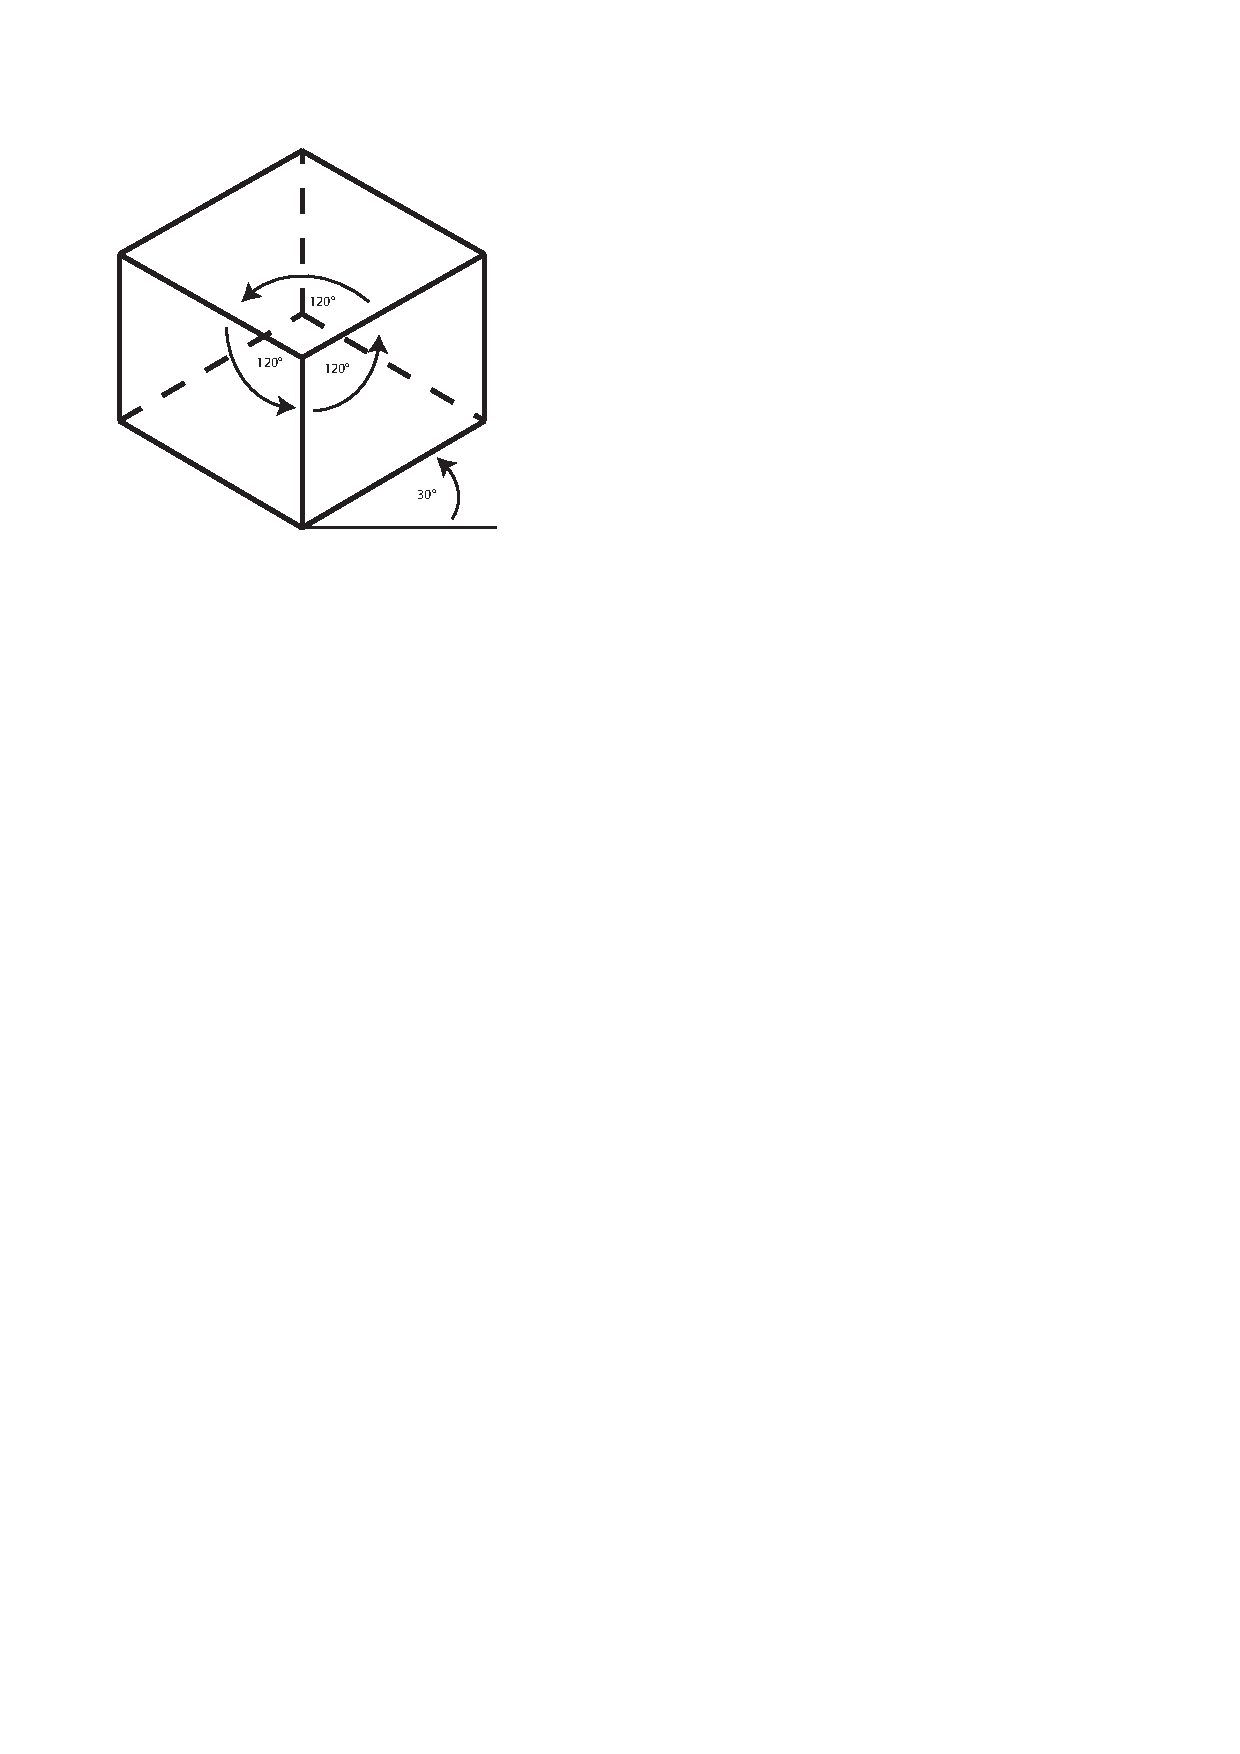
\includegraphics[clip=true,trim=0 205mm 100mm 0]{thesis-isobox}
	\caption{Isometric projection}
	\label{isometric}
\end{figure}

\subsection{Isometric camera}
The camera is top down, but tilted by 45 degrees in both directions. The diagonals therefore should be at 30 degrees, but due to the irregular aliasing of these diagonals on the bitmap grid the practical approach is slightly different. Figure \ref{isoangle} shows the problematic bitmap grid as well as the solution. The image is rotated by 45 degrees and then the aspect ratio is changed to 2:1. The result are regular 2pixel stairs forming diagonals in about 26.565 degrees\footnote{\begin{math}\arctan \frac{1}{2} \approx 26.565\si{\degree}\end{math}}. The side effect of this change is complete elimination of trigonometry from the projection mathematics further improving the rendering performance.

\begin{figure}[htp]
	\centering
	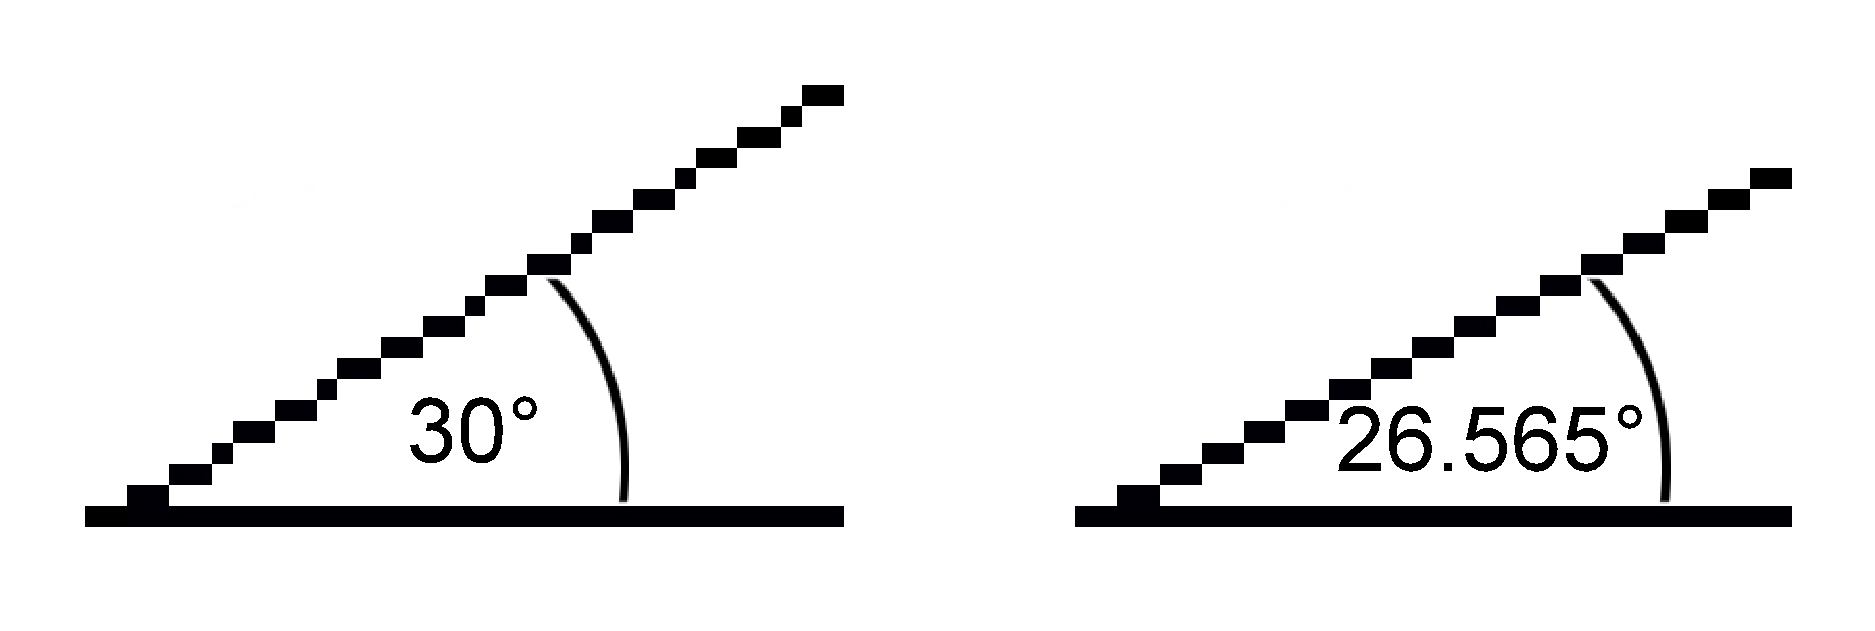
\includegraphics[width=0.7\textwidth]{thesis-angles}
	\caption{Isometric projection angle}
	\label{isoangle}
\end{figure}

\subsection{Example games, brief history}
The first game using isometric graphics was Zaxxon released by SEGA in 1982\cite{zaxxon} (see Figure \ref{zaxxon}). This new approach allowed to display 3D scene without the need for hardware accelerated 3D rendering. The same graphic style was later used in many other games, especially genres where the player overviews the scene from the top. \emph{Dune II} released in 1992\cite{dune2} used direct top-down camera. To improve the visual appeal \emph{Warcraft: Orcs \& Humans} released two years later\cite{blizzardlegacy} tilted the camera slightly in one direction. Later games in the strategy genre\footnote{1990s classics including turn-based strategy \emph{Civilization II}\cite{civ2}, real-time strategy \emph{Age of Empires}\cite{ageofempires} and business simulator \emph{Transport Tycoon Deluxe}\cite{ttd}} fully adapted the isometric projection. These strategies often divided the map to regular tiles that limited the player actions but made collision detection and other game mechanics very simple. This design outlived the slow hardware with no graphic acceleration and is still popular both among independent developers with limited resources and in environments where hardware acceleration is not granted\footnote{Typically browser games discussed later.}. When 3D acceleration became affordable, focus of game development shifted to full 3D rendering. Although the player could be given full control of the camera, many games lock the camera in the same angle as is the isometric camera in order to avoid player confusion. Provided combination of realistic look of 3D rendered scene with perspective, shadows etc. and a clear overview of the scene defined by the isometric camera angle has proven to be optimal for wide array of games. Prime example be professionally played \emph{Starcraft 2}\cite{sc2} that does allow camera rotation, but the camera automatically returns to the original position afterwards.

\begin{figure}[htp]
	\centering
	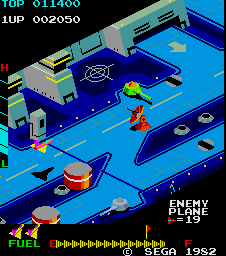
\includegraphics{zaxxon}
	\caption{Isometric graphics in original arcade version of Zaxxon\cite{zaxxon}}
	\label{zaxxon}
\end{figure}

\section{Web graphics and HTML5}
Web applications on the client side can rely only on the browser application and its capabilities. No middleware directly accessing hardware is guaranteed. Therefore the browser games\footnote{Games played on a web page displayed in the browser.} draw graphics to some element in the HTML page. Prior to the version 5 of the HTML standard, the games almost exclusively used Flash and required the client browser to have Adobe Flash Player plug-in installed\cite{flashplayer}. With the broad adoption of HTML5, new options presented themselves. Two new elements to display graphics allow to stop making any assumptions about the client other than whether it supports HTML5.

\subsection{Canvas, usage in games}
The \texttt{canvas} element is very similar to the canvas objects in other programming environments\footnote{E.g. classes \texttt{System.Windows.Controls.Canvas} in .NET framework\cite{net_canvas} or \texttt{java.awt.Canvas} in the Java platform\cite{java_canvas}}. It allows to directly draw to the canvas bitmap using JavaScript functions. Even though this approach is straight forward, some disadvantages arise when applied. Most noticeable is that when an object is being changed, everything that even partially covers it has to be re-drawn as well even if it stays unchanged. Also when drawing several objects that appear behind and in front of each other, these need to be carefully drawn in a correct order so the overlaps are correct and the illusion of space remains unbroken.

Due to the similarity to other environments there is already large variety of game engines implemented on the \texttt{canvas} element. Used underlying element is often reflected in the engine name\footnote{E.g. \emph{Canvace}\cite{canvace} or \emph{Canvas Engine}\cite{canvasengine}}, but other take \texttt{canvas} usage as a matter of course\footnote{E.g. \emph{enchant.js}\cite{enchantjs} or proprietary \emph{Isogenic Game Engine}\cite{isogenic}}.

\subsection{SVG}
The \texttt{svg} element is very different as it displays given SVG\footnote{Scalable Vector Graphics}, a vector image described in a markup language of the same name. It can also be dynamically manipulated with JavaScript, but the approach is fundamentally different. Elements are added to the DOM\footnote{Document Object Model} as if only standard HTML was used. Instead of redrawing the whole image or a part of screen, individual objects can be added, removed or changed. This makes for example an animation of an object much more straight forward. User interaction handling is also easier since event handlers can be hooked onto the elements representing the objects.

Even though browsers used to support static SVG for a long time, not until HTML5 did they support dynamic in-line SVG\cite{w3_html5}. This is now available with the previously mentioned element. Since rendering the markup language is much more complicated than simple dumping the canvas bitmap on the screen, the browser support is delayed and also more sensitive to performance problems. Drawing to the canvas may take a lot of JavaScript execution time, but in the end the display of the element takes amount time only effected by the size of the canvas, not complexity of its content. Creating large SVG will take similar time, but then rendering it on the screen will take browser another time.

\chapter{Suggested solution / design}
\label{solution}
As it was discussed earlier, \texttt{canvas} based engines for browser games are quite common. Why is that there are no game engines based on \texttt{svg}? W3Schools in a chapter about HTML5 \texttt{svg} element warn that it, unlike the \texttt{canvas} element, is not suitable for game applications\cite{html5svg}. However is it possible to use an inline SVG to draw game graphics instead of the standard canvas approach? With the event handling support it should be even more suitable and furthermore manipulation with specific objects in a drawn scene should make the subsequent scene updates much easier.

Suggested idea is to make an attempt to create such engine. An engine that will be able to ask for data that describe area actually on screen. Retrieved data will transform to their visual representation and render to the \texttt{svg} element. Of course all of this and the user interaction handling needs to be separated from the actual implementation for the engine to be generally usable by different end applications. To keep the scope focused enough so the implementation can provide some actually helpful functionality for the end application developer rather than just another abstraction layer over the SVG DOM, the engine shall be limited to render isometric tile-based graphics that are, as discussed earlier, still popular among both developers and players. This limitation allows the implementation to encapsulate all logic regarding isometric coordinate transformation.

\section{Data retrieval}
Although in case of a single-player game\footnote{Game for only one player with no interaction with other people playing the same game.} the data can be completely generated and stored on the client instance, remote data retrieval needs to be supported as well. Furthermore since even single-player games are likely to store level map data in some common storage, the remote data access is expected to be prevalent use in eventual implementation usages. To keep the data transfer down, the data provider\footnote{Hereinafter referred to as the server.} is given an option to decide either to send full data matrix of requested area in the response or send only data of the tiles that changed since last request if the matrix of actually useful data would be too sparse. The former approach needs less data per tile since only the coordinates of a top left corner of the requested area needs to be included in the response since all other can be calculated from the response data. On the other hand the latter approach coordinate for each tile. Of course the efficiency of both ways depends on many other things. How thick or thin the client is hence whether the server keeps track of individual client request history. The tile data size to the two-integer coordinates ratio is also important as well as the speed of map data change. Nevertheless both approaches find it's use and the engine has to be able to process data presented in both formats.

The tile data record may contain more information than it is necessary to deduce the tile visual representation hence only a subset of this data record should be passed to the general map data requests to further lower the bandwidth usage. Then there must be a way to retrieve the rest of the tile data record for game logic purposes though. To provide this channel, engine has to implement a full data request for a tile involved in advanced operations.

\section{Sprites}
The standard way of making 2D games is to draw small images of objects and then compose the scene using these images. This way the object can be animated easily by replacing said image with next animation frame image. For performance reasons all these sprites are compiled to a single image called sprite-sheet.\cite{pagella} The graphics engine needs to be able to draw a sub-selection of the sprite-sheet image. When working with HTML5 \texttt{canvas} element, JavaScript function \texttt{CanvasRenderingContext2D.drawImage(img, sx, sy, swidth, sheight, x, y, width, height)} does exactly that\cite{canvasdrawimage}. First set of of coordinates and dimensions determines which part of the source image will be drawn. Second set of coordinates and dimensions then determines the target location on the canvas.

When using SVG, no such a straightforward and convenient way is available. To display a section of an image, one needs to create a pattern from it and position it using a negative coordinates. The pattern must use \emph{objectBoundingBox} units so it doesn't shrink the whole sprite-sheet in the target element. Then an SVG element (usually polygon) using this pattern can display desired selection of an image. The limitation of this approach is that all elements using the same pattern must have synchronous animation, what usually doesn't look too organic in the result. On the other hand it nicely emulates the early 90s era of gaming.

The more natural approach for \texttt{svg} would be having sprite-sheet defined as a separate SVG file containing vector sprites defined by SVG markup. Although this is certainly possible, vector graphics are not as widely used as bitmaps in the game development.

Beside \texttt{canvas} the SVG allows to use animated GIFs\footnote{Graphics Interchange Format is an image format that allows to contain a series of images that are displayed in sequence to show an animation\cite{gifstandard}.} as sprites. The creation of sprites or even sprite-sheets this way is more complicated. However when using sprites that are already animated, execution time needed to animate static tiles can be saved. The amount of saved time of course depends on the browser implementation and its support of said GIFs. In some cases this may even yield worse result than using static image formats.

\chapter{Used technologies}
\label{tech}

\section{Engine}
The graphics engine is being run on the client and hence all technologies used in it are based around JavaScript.

\subsection{Browser support of HTML5 SVG element}
HTML5's \texttt{svg} element as such is well supported by modern browsers\cite{html5svg}, but there are some difficulties with the implementation details in different browsers. A striking example be Internet Explorer that entirely lacks support of \texttt{foreignObject} SVG element that normally allows to nest HTML in the SVG image\cite{ieforeignobject}.

\subsection{SVG manipulation JavaScript libraries}
The contents of the \texttt{svg} element can be manipulated directly via JavaScript, but like regular HTML DOM manipulation it is laborious and ends up with lots of repetitive code. To eliminate this drawback there are several JavaScript libraries that provide abstract layer over the SVG markup. Most of them are open source.

A pioneer among these libraries is \emph{Raphaël}. The projects puts emphasis on wide browser support including archaic Internet Explorer version 6.0 \cite{raphael}.

\emph{Raphaël}'s rewrite, \emph{Snap.svg} is not held back by compatibility to obsolete browsers and so it can support features like masking, clipping, patterns, full gradients, groups\cite{snap}. Snap.svg is quite popular among front-end developers who typically create animation based on static SVG for web sites\cite{snapusage}. When working with SVG elements and their attributes are represented as string values. This may be perfect for mentioned application, but when creating all of the content dynamically, this involves a lot of string concatenation in the end, which is far from ideal in intended use.

Next library called simply \emph{svg.js} takes more object oriented approach\cite{svgjs} that is more suitable for this project. The project is modularized so for a production environment can be built with only the functionality that is really used to decrease script size. There are also quite a few additional modules providing extra functionality that might prove useful.

Another popular project called \emph{D3.js} does not limit its scope to SVG and approaches the DOM manipulation in a similar manner to \emph{jQuery}\cite{d3js}. Emphasis on querying the DOM, that is very performance demanding once the DOM has a large amount of elements, makes this project not suitable as well.

There are of course other libraries, but since the game developer using the engine will have to work with given SVG manipulation library to some extent, commonly used library with good documentation may make his use of the engine much easier. All considered, the \emph{svg.js} project was selected to serve as a SVG markup markup manipulation API.

\subsection{General utility JavaScript libraries}
Other general purpose JavaScript libraries are used to keep the actual engine code clean and readable. Like previously discussed libraries, these are open source as well and use non-restrictive licenses.

To help manage the JavaScript application structure is used library \emph{require.js} that allows to define modules and dependencies between them. Then it makes sure all files containing required modules are loaded prior to their usage. \cite{requirejs} This approach eliminates many of flaws of JavaScript as a language, particularly declaration scope confusion and possible redeclaration of variables and dependency on functions or variables that may not be declared yet.

Some very limited HTML manipulation is simplified using \emph{jQuery} library. Since the engine does not work with HTML out of the \texttt{svg} element the usage is rather minimal, mostly to access element properties in a unified fashion\footnote{Even something as simple as getting element's actual width can be quite laborious to get working across browsers without \emph{jQuery}.}. Since the display of game scene can generate quite a lot of elements, querying them, the main point of \emph{jQuery}\cite{jquery}, has to be done with performance in mind.

Automatic tests of the engine API are written using the \emph{Jasmine} framework. It allows to define test cases and expected behaviour\cite{jasmine}. Out of the box can these tests be run in the browser like the engine itself. Using the \emph{Karma} test runner the tests also can be integrated to the \emph{maven}\footnote{Maven is a build automation tool\cite{maven} used in this project mostly due to the demo back-end written in Java.} build process\cite{karma}.

\section{Other technologies used in the demo game}
The demo application created to demonstrate capabilities of the engine combines it with other technologies just like real world application would. Other application may change completely different set of dependencies, therefore the ones used in the demo application in no way bound to the actual engine.

\subsection{JavaScript objects provided by browsers}
Since the engine itself is abstracted from actual data source and format, the browser support for network communication and serialization is not needed until the specific game implementation.

For obtaining data from the server uses the demo application \texttt{XmlHttpRequest}, a JavaScript object widely supported by browsers\cite{xhr}. It allows to create an asynchronous HTTP request with a callback when the response is obtained.

To parse the JSON\footnote{JavaScript Object Notation data format} responses to a JavaScript object is used the \texttt{JSON} JavaScript object specified by ECMAScript 5.1 and also supported by modern browsers\cite{json}.

\subsection{RESTEasy}
RESTEasy is a JBoss project allowing to create a web service with parametrized URLs mapped to methods\cite{resteasy}. This service can very easily  provide RESTful\footnote{RESTful service meets all requirements defined by Representational State Transfer architecture, that is mainly unified access to creation, reading, update and deletion of provided resource\cite{fielding}.} management API, hence the project name. Jackson JAX-RS providers\cite{jackson} are used instead of the default JSON serializer to allow the service return custom Java objects with no additional annotations serialized to JSON. This framework was selected due to the simplicity of creating a service that provides access to the pseudo randomly generated model of the demo application.

\subsection{AppEngine API}
Google App Engine is a cloud hosting service provided by Google. The engine demo application was hosted on this service for demonstration purposes and so the project had to contain piece of appropriate configuration. With generously limited bandwidth is the service free of charge. \cite{appengine}

\chapter{Implementation}
\label{implementation}
Important part of the engine implementation is reusability and therefore abstraction of all details of any specific game. Anything that would lead to these specifics is performed via calling handler functions on objects providing the specific game implementation. Figure \ref{classdiagram} shows dependencies among the JavaScript modules.

\begin{figure}[htp]
	\centering
	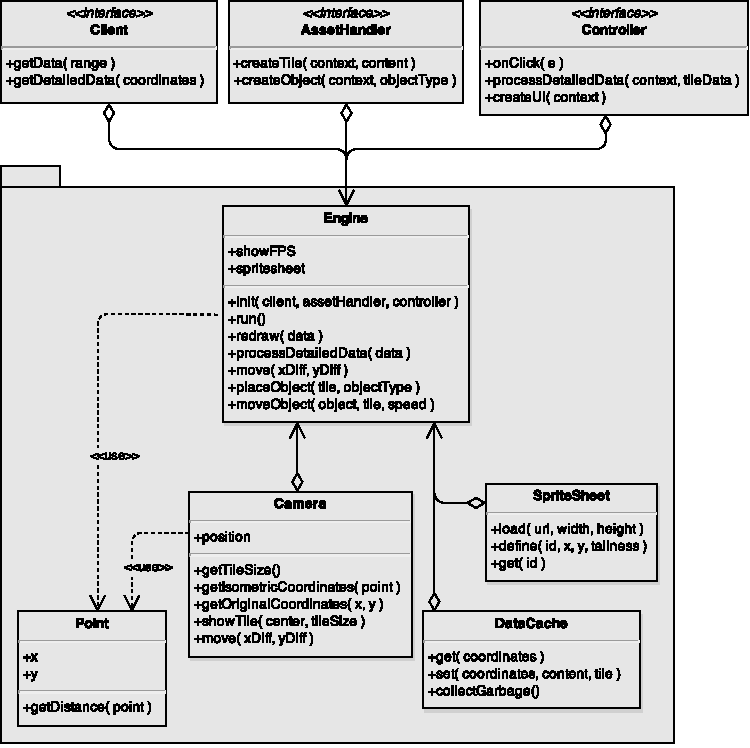
\includegraphics[width=\textwidth]{thesis-classdiagram}
	\caption{Diagram of the JavaScript modules}
	\label{classdiagram}
\end{figure}

\section{Viewport population and data fetching}
To populate the screen with tiles, data describing each of the tiles that will be displayed on the screen need to be obtained. That is performed via an asynchronous call to the client object that will in return call asynchronous callback on the engine after it obtains or creates the requested data. These data can be continuous array of tile content values or if the client determines that only a few tiles changed, only content and coordinates of these changed tiles can be returned. This will save data traffic when repeatedly requesting updates of the same area.

\begin{figure}[htp]
	\centering
	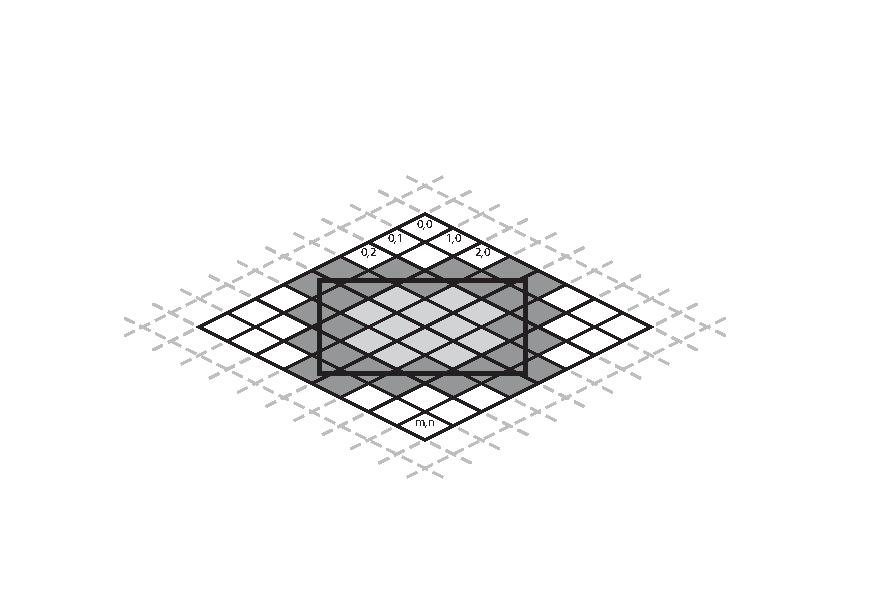
\includegraphics[clip=true,trim=20mm 17mm 20mm 23mm]{thesis-isodata}
	\caption{Data needed to fill a rectangle viewport}
	\label{isodata}
\end{figure}

\section{Object stacking and verticality}

\section{Features I did not implement with reasoning why not}

\chapter{Testing and measurement}
\label{testing}

\section{Performance on desktop and mobile devices}
Mobile devices were probably a long shot, even desktop browsers have vast differences in performance - in chrome everything runs nicely, Firefox is barely usable and Internet Explorer 11 is absolutely useless.

\chapter{Conclusion}
Evaluation of the results with emphasis on my contribution from the point of view of a wider context.
Future work, possible improvements - missing features, React.js to optimize the DOM manipulation.

\bibliographystyle{csplainnat} % sets plain bibliography style  
\bibliography{sources}     % BibTeX database file  

\appendix
\chapter{How to use my engine for your game}
The engine provides API makes the viewport manipulation very easy. The use of this API is demonstrated in the \href{https://github.com/vit-svoboda/svg-engine/tree/master/src/main/webapp/Scripts/game}{sample application}.

\section{Data feed}
Data describing what should be displayed are provided to the engine through an object passed as a first parameter of engine.init method. When engine needs data, methods getData or getDetailedData are called. This data can be obtained from a remote server using HTTP requests, stored in the client memory and passed directly or in any other way suitable for the given game.

\section{Asset management}
To give the game implementation power over what is displayed in place of data discussed earlier, everything displayed is translated using an object passed as a second parameter of the engine.init method. This translation is performed via methods createTile or createObject where the SVG drawing context is provided. Result is placed on the corresponding place in the viewport.

\section{UI handling and game logic}
The third object passed to the engine.init method is responsible for handling user interaction. method createUi is responsible for the standard UI displayed all the time, method processDetailedData is a handler for detailed tile data once it is obtained and method onClick is a handler for any tile or object clicked. Here most of the user interaction needs to be handled. Very little boundaries are given to other interaction implementation though.

\end{document} 